\documentclass{article}
\documentclass{standalone}
\usepackage{graphicx} % Required for inserting images
\usepackage{graphicx} % Required for inserting images
%\usepackage[left=0.5in, right=0.5in, top=0.5in, bottom=0.5in]{geometry}
%\usepackage[left=1.5cm, right=1cm, top=0.5cm, bottom=1.5cm]{geometry}
\usepackage[left=1.5cm, right=1.5cm, top=0.5cm, bottom=1.5cm]{geometry}
\usepackage{amsmath}
\usepackage{amssymb}
\usepackage{amsfonts}
\usepackage{amsthm}
\usepackage{ulem}
\usepackage{bm}
\usepackage{tikz}
\usepackage{enumitem}

\date{}

\begin{document}
\fontsize{13}{15} \selectfont %This is 13pt text with 15pt line spacing.

\begin{center}
 \text{Potterhouse School. \hspace{1cm} Year 6 Math - Mixed Task 5.} \qquad \\ 
\end{center} \\ 

Name: ...........................................................  \hspace{0.5cm}  Date: ....................... \hspace{0.5cm}  Class: ......\hspace{0.5cm} [20 marks]

\par
\vspace*{5pt} 
\textit{(You must show your working including the times tables of the divisors and multipliers.)  }
%\vspace{5pt}

\begin{center}
    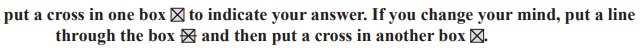
\includegraphics[width=15cm]{Year_6_Mixed_Tests/Xx.png}
\end{center}
 \\

 \begin{enumerate}
 
\item \quad \( 6532 \div 24 \)   \hspace{2cm} [2 marks] 
\vspace{90pt}
\hline
\vspace{5pt}

\item \quad \( 2436 \times 34 \) \hspace{2cm} [2 marks]
\vspace{90pt}
\hline
\vspace{5pt}

\item \quad \text{Which one is a prime number? Give a reason. } \hspace{2cm} [2 marks]
\vspace{30pt}

\begin{center}
\begin{tabular}{c@{\hspace{3cm}}c@{\hspace{3cm}}c@{\hspace{3cm}}c}
  23 & 60 & 48 & 51 \\  
  
\includegraphics[width=1cm]{cross.png} & 
  
\includegraphics[width=1cm]{cross.png} & 
  
\includegraphics[width=1cm]{cross.png} & 
  
\includegraphics[width=1cm]{cross.png} \\
\end{tabular}
\end{center}
\hline
\vspace{10pt}

\item \quad \text{ Which one is a cube number? Give a reason. } \hspace{2cm} [2 marks]
\vspace{30pt}

\begin{center}
\begin{tabular}{c@{\hspace{3cm}}c@{\hspace{3cm}}c@{\hspace{3cm}}c}
  75 & 64 & 18 & 6 \\
  
\includegraphics[width=1cm]{cross.png} & 
  
\includegraphics[width=1cm]{cross.png} & 
  
\includegraphics[width=1cm]{cross.png} & 
  
\includegraphics[width=1cm]{cross.png} \\
\end{tabular}
\end{center}
\hline
\vspace{10pt}

\item \quad \text{ Which one is a square number? Give a reason. } \hspace{2cm} [2 marks]
\vspace{30pt}

\begin{center}
\begin{tabular}{c@{\hspace{3cm}}c@{\hspace{3cm}}c@{\hspace{3cm}}c}
  24 & 25 & 26 & 27 \\
  
\includegraphics[width=1cm]{cross.png} & 
  
\includegraphics[width=1cm]{cross.png} & 
  
\includegraphics[width=1cm]{cross.png} & 
  
\includegraphics[width=1cm]{cross.png} \\
\end{tabular}
\end{center}
%\hline
\vspace{10pt}

\item \text{ Write these numbers in order of size. Start with the smallest. } \hspace{2cm} [2 marks] \\
\begin{center}
4.045\hspace{2cm}4.054\hspace{2cm}45\% \hspace{2cm} \( \displaystyle \frac{4}{5}\) 
\vspace{50pt}

.......\hspace{2cm}.....\hspace{2cm}.....\hspace{2cm}.....  \\
\end{center}
\hspace {2cm} Smallest

\vspace{10pt}

\hline
\vspace{10pt}

\item \quad \text{ Fill in A, B, C and D in the number line below. } \hspace{2cm} [2 marks]
\vspace{10pt}

% Negative number line 

\begin{tikzpicture}[x=0.8cm]  % Set the x unit vector length to 0.8cm
    % Draw the main line
    \draw[->] (-10,0) -- (10,0);
    
    % Draw tick marks and labels
    \foreach \x in {-10, -8, ..., 10} {
        \draw (\x,-0.1) -- (\x,0.1);
        % Omit labels at positions -7, -3, 2, and 8 to leave them blank for letters
        \ifnum\x=-8 \else \ifnum\x=-6 \else \ifnum\x=-2 \else 
        \ifnum\x=2 \else \ifnum\x=4 \else  \ifnum\x=8 \else 
            \node[below] at (\x,-0.2) {$\x$};
        \fi\fi\fi\fi\fi\fi
    }
    
    % Draw letters 'A', 'B', 'C', and 'D' at positions -7, -3, 2, and 8
    \node[below] at (-8,-0.2) {A};
    \node[below] at (-2,-0.2) {B};
    \node[below] at (4,-0.2) {C};
   % \node[below] at (8,-0.2) {D};
    
\end{tikzpicture}
\vspace{70pt}

\hline
\vspace{5pt}

\item \quad \text{Write} \bm{\mathit{46378}} \text{in words. } \hspace{2cm} [2 marks]
 %\text{(7) Write} \text{\textit{$\bm{38127}$}} \text{in words. } 
 \par
 \vspace{30pt}

\noindent \dotuline{\hspace{17cm}} \\
\par
\noindent \dotuline{\hspace{17cm}} \\
\vspace{10pt}
\hline
\vspace{10pt}

\item \quad \text{Write} \textit{\textbf{seventeen million, five hundred and thirty-two thousand, }} \\
\textit{\textbf{ nine hundred and twenty-three}} \text{in digits.} \hspace{2cm} [2 marks]

 
 \par
 \vspace{50pt}
 ..............................................

 \vspace{20pt}
 \hline
 \vspace{10pt}

\item (a) \quad \( 5^{2} + 14 \div (5 + 2) \) \hspace{2cm} [1 mark]
\vspace{90pt}
\hline
\vspace{10pt}

(b) \quad \( 7 + 3^{3} \times (8 + 2 ) \) \hspace {2cm} [1 mark]
\vspace{40pt}
%\hline
\vspace{10pt}

\end{enumerate}
\end{document}